\chapter{Inhoudelijk beheer} \index{inhoudelijk beheer}
\section{Boeken}
Structuur van boeken beheren.
\subsection{Book-module} \index{book-module}
De Book-module is geschikt voor het maken van hi\"irarchische pagina's zoals
handboeken, 'veel gestelde vragen' (FAQs) of verzamelingen van verwijzingen naar sites (site resource guides).
Een boekdocument kan hoofdstukken, paragrafen, subparagrafen, enz. hebben. Auteurs met de juiste
toegangsrechten kunnen pagina's aan een gezamenlijk boek toevoegen en deze in het bestaande document
 plaatsten door ze aan het inhoudsmenu toe te voegen.
\\
Boeken hebben onderaan de pagina's navigatie-links \index{navigatie-links} om
door de pagina's van het boek te bladeren. Deze verwijzen naar vorige en volgende pagina's en naar de bovenliggende pagina.
Aanvullende navigatie is beschikbaar door op de pagina blokbeheer het blok
boeknavigatie \index{bloknavigatie} in te schakelen.
\\
Gebruikers kunnen de link printervriendelijke versie \index{printversie} onder
de boekpagina gebruiken om een printervriendelijke versie van de pagina en al haar onderdelen weer te geven.
\\
Gebruikers met de toegangsrechten Boekstructuren beheren kunnen pagina's van
ieder inhoudstype aan een boek toevoegen door het betreffende boek te selecteren tijdens het
bewerken van de pagina of door het tabblad Structuur te gebruiken.
\\
Beheerders kunnen op de pagina Boekbeheer een lijst van boeken weergeven.
Op de pagina Structuur kunnen paginatitels en de paginastructuur gewijzigd worden.
\\
Lees voor meer informatie het online-handboek over de Book-module.
\subsection{Toegangsrechten instellen} \index{toegangsrechten}
Met toegangsrechten kunt u bepalen wat gebruikers op de site kunnen doen.
\begin{itemize}
\item toegang tot printervriendelijke versie
\item inhoud aan boeken toevoegen
\item Boekstructuren beheren
\item nieuwe boeken aanmaken
\end{itemize}
\subsection{Instellingen}
\begin{itemize}
\item Toegelaten boekstructuurtypen
\item Standaard subpaginatype
\end{itemize}

\section{Inhoud}
De inhoud van de website weergeven, wijzigen en verwijderen.
 \begin{figure}[!h]
    \centering
   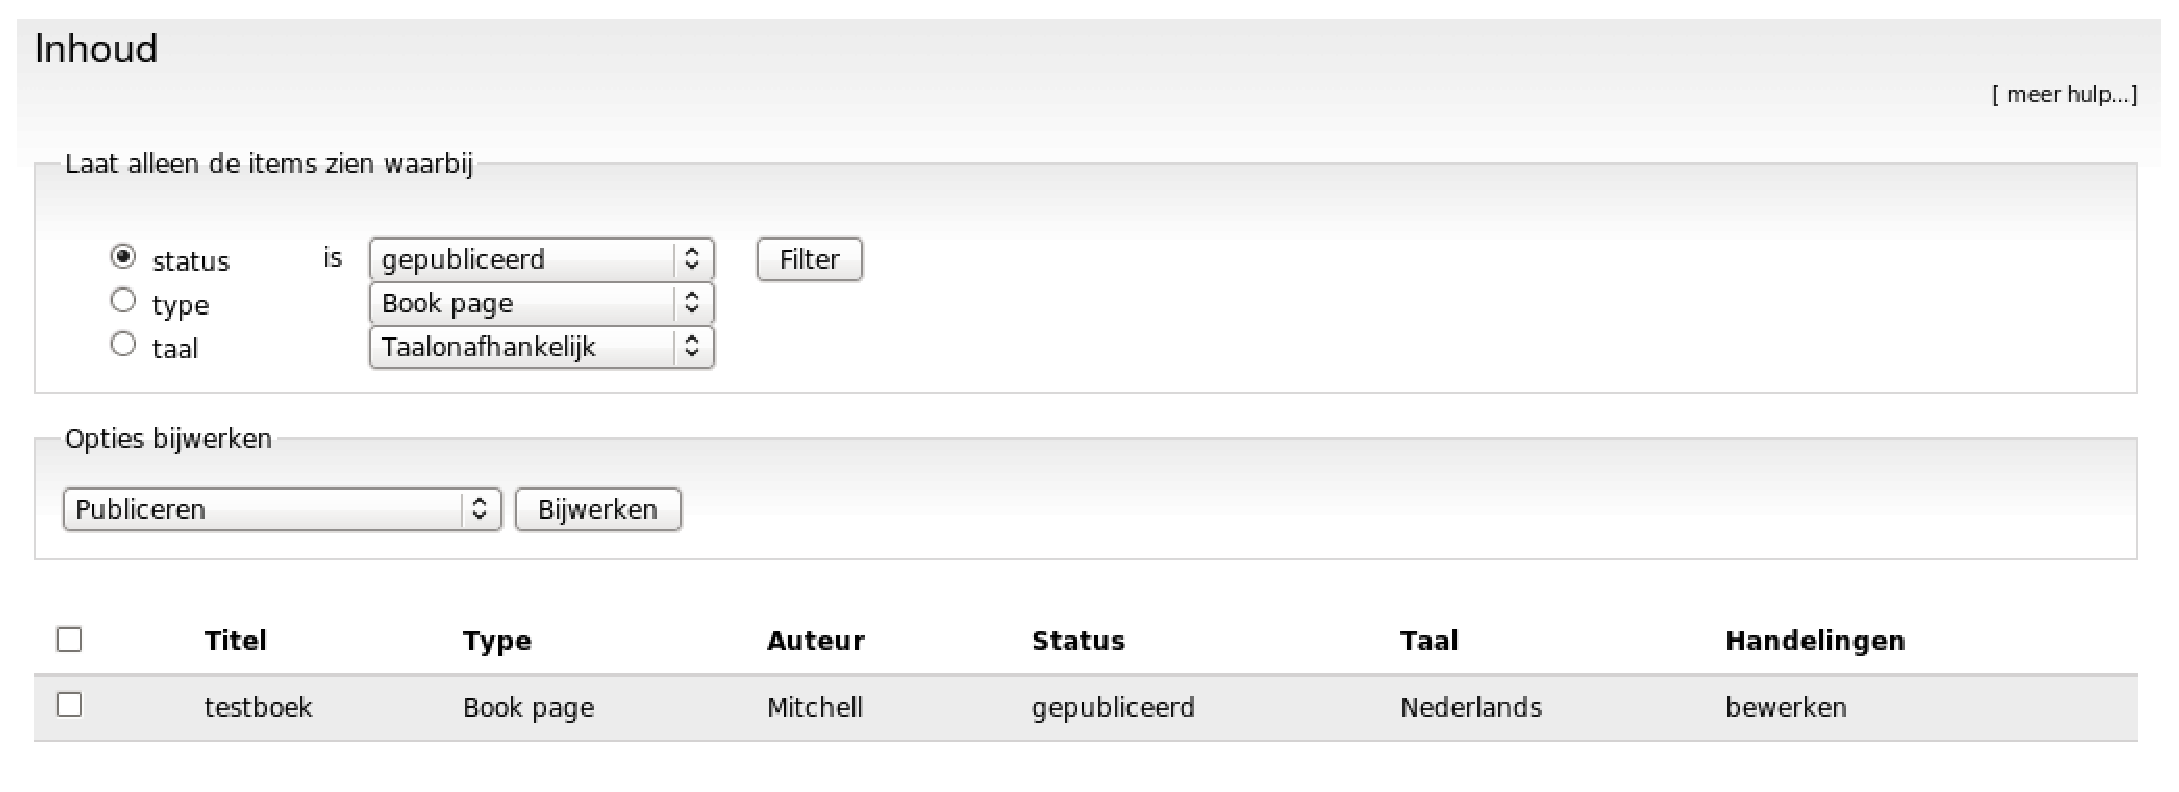
\includegraphics[scale=0.3,angle=0]{inhoud}
   \caption{Inhoud.\label{white}}
 \end{figure}
 \subsection{Node} \index{node}
De Node-module \index{node-module} beheert de inhoud van de site en slaat alle
ingevoerde pagina's (ongeacht het type) als 'node' op. De node bevat naast de publicatie opties (of een node gepubliceerd is, op de voorpagina zichtbaar is, bovenaan een
lijst wordt weergegeven) ook basisinformatie over de auteur van de pagina. Revisie-informatie van de node is
optioneel beschikbaar. Voor meer mogelijkheden wordt de Node-module vaak met andere modules uitgebreid.
\\
Iedere door gebruikers toegevoegde pagina op de website een node van een bepaald inhoudstype. Inhoudstypen
worden gebruikt om verschillende soorten pagina's of gegevenssoorten de defini\"eren. In een Inhoudstype zijn
eigenschappen vastgelegd zoals inclusief de paginatitel, type en aantal invoervelden en beschrijvingen bij de
invoervelden. Verder kunnen per inhoudstype verschillende standaard Publicatieopties en werkschema's worden ingesteld.
Standaard kent Drupal twee inhoudstypen: \index{inhoudstypen} Pagina
\index{pagina} en Verhaal \index{verhaal}. Op de pagina inhoudstypen kunnen
inhoudstypen worden toegevoegd. Ook kunnen typen worden toegevoegd door kern-modules, uitbreidingsmodules en zelf ontwikkelde modules.
\\
Op de pagina Inhoudelijk beheer vindt u een overzicht van de inhoud van de website en kunt u deze beheren.
De pagina Instellingen voor inzendingen bevat enkele instellingen voor de weergave van inzendingen.
De Node-module brengt voor ieder inhoudstype een aantal instellingen met zich mee die per rol op de
pagina Toegangsrechten kunnen worden ingesteld.

\section{Inhoudstypen}
Inzendingen per inhoudstype beheren zoals standaard status, aangeraden voor
voorpagina, enz.
\subsection{Lijst}
De onderstaande fig. geeft alle inhoudstypen op de site weer. Alle inzendingen
op de site zijn exemplaren van de onderstaande inhoudstypen.
 \begin{figure}[!h]
    \centering
   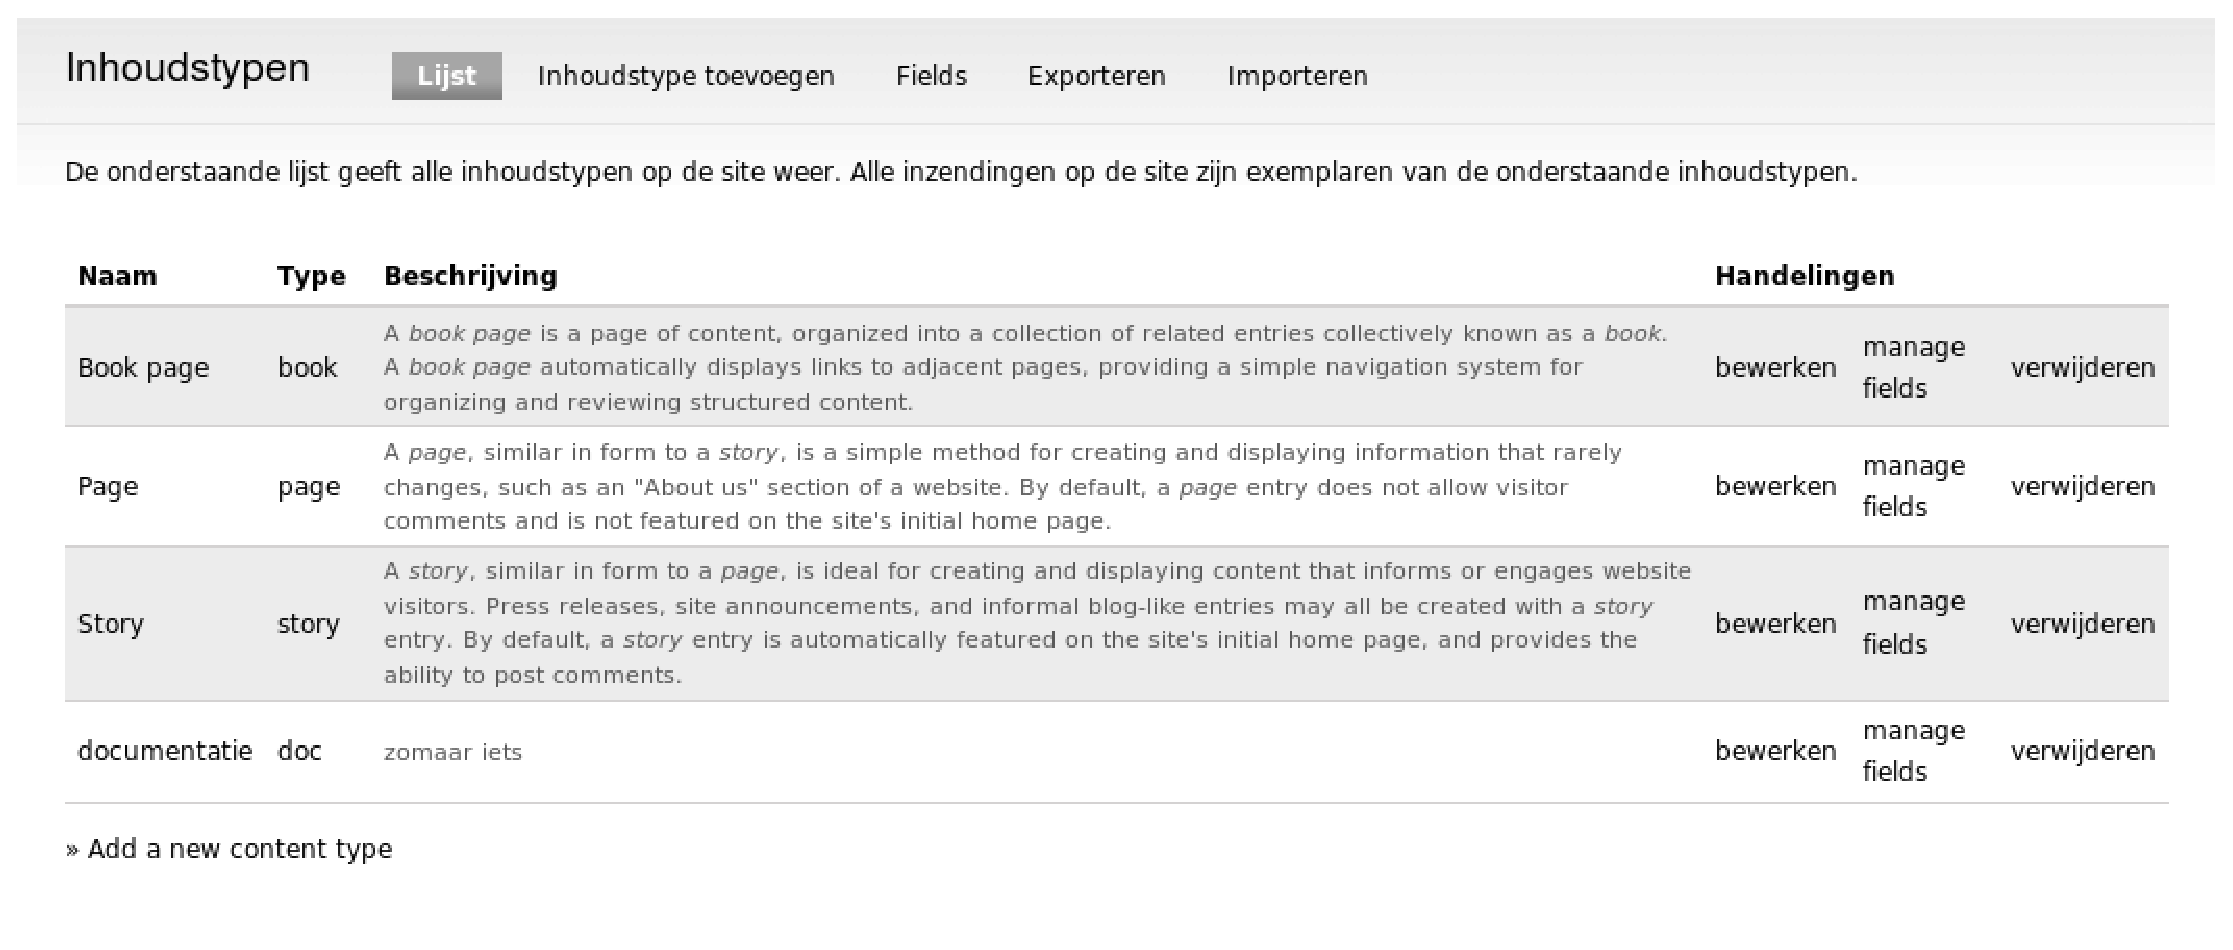
\includegraphics[scale=0.3,angle=0]{inhoudstypen-lijst}
   \caption{inhoudstypen-lijst.\label{white}}
 \end{figure}

\subsection{Inhoudstype toevoegen}
Maak een nieuw inhoudstype aan door een voor mensen begrijpelijke naam, een
machinaal leesbare naam en de overige relevante velden op deze pagina in te vullen.
Nadat een inhoudstype is aangemaakt kunnen gebruikers hiermee inhoud aan de site toevoegen.
\begin{figure}[!h]
    \centering
   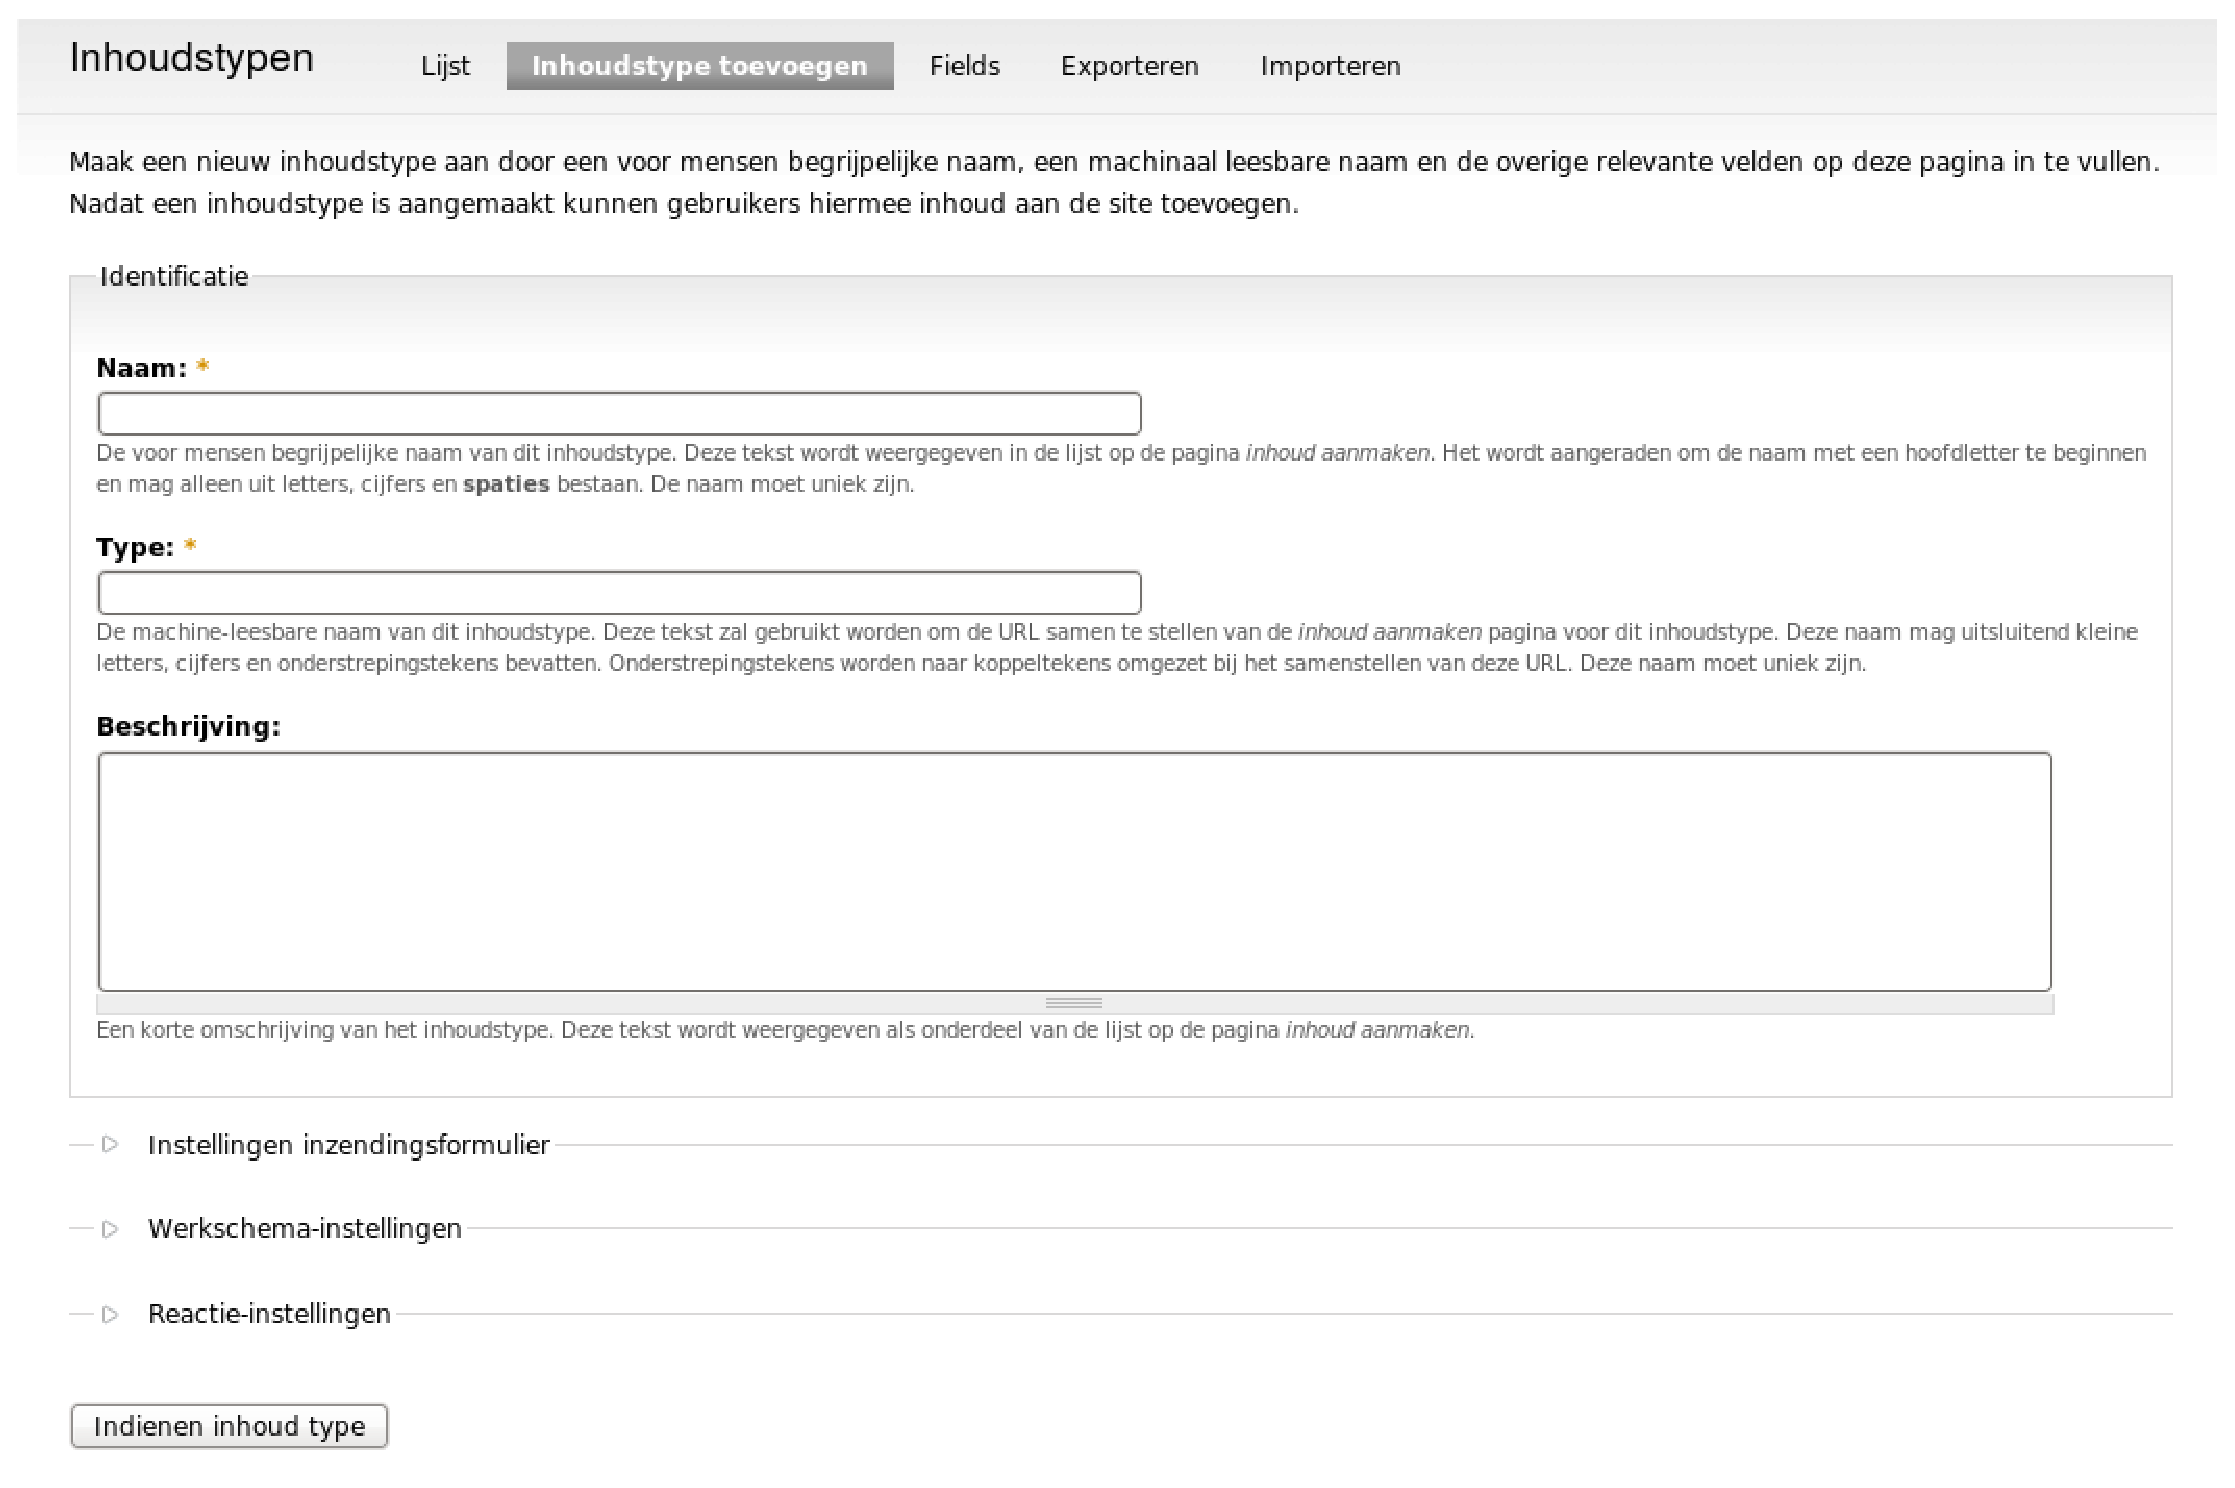
\includegraphics[scale=0.3,angle=0]{inhoudstypen-invoegen}
   \caption{inhoudstypen-invoegen.\label{white}}
 \end{figure}

\subsection{Fields}
\begin{figure}[!h]
    \centering
   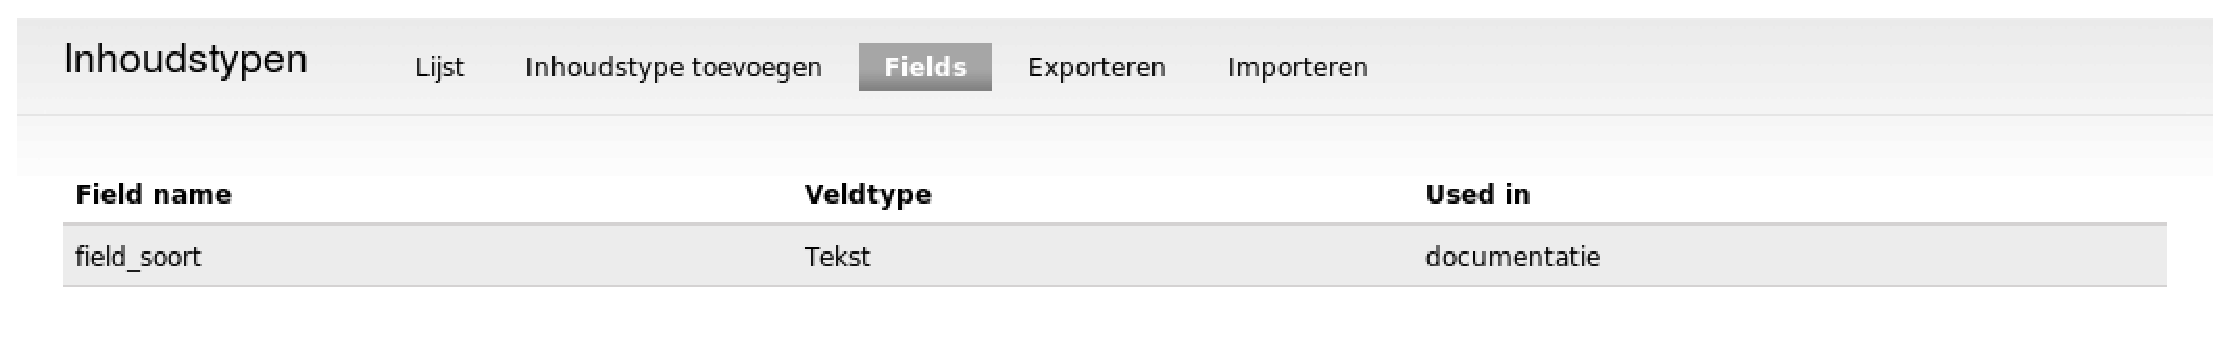
\includegraphics[scale=0.3,angle=0]{inhoudstypen-fields}
   \caption{inhoudstypen-fields.\label{white}}
 \end{figure}

\subsection{Exporteren} \index{exporteren}
This form will process a content type and one or more fields from that type and
export the settings. The export created by this process can be copied and pasted as
an import into the current or any other database. The import will add the fields to
an existing content type or create a new content type that includes the selected fields.
\begin{figure}[!h]
    \centering
   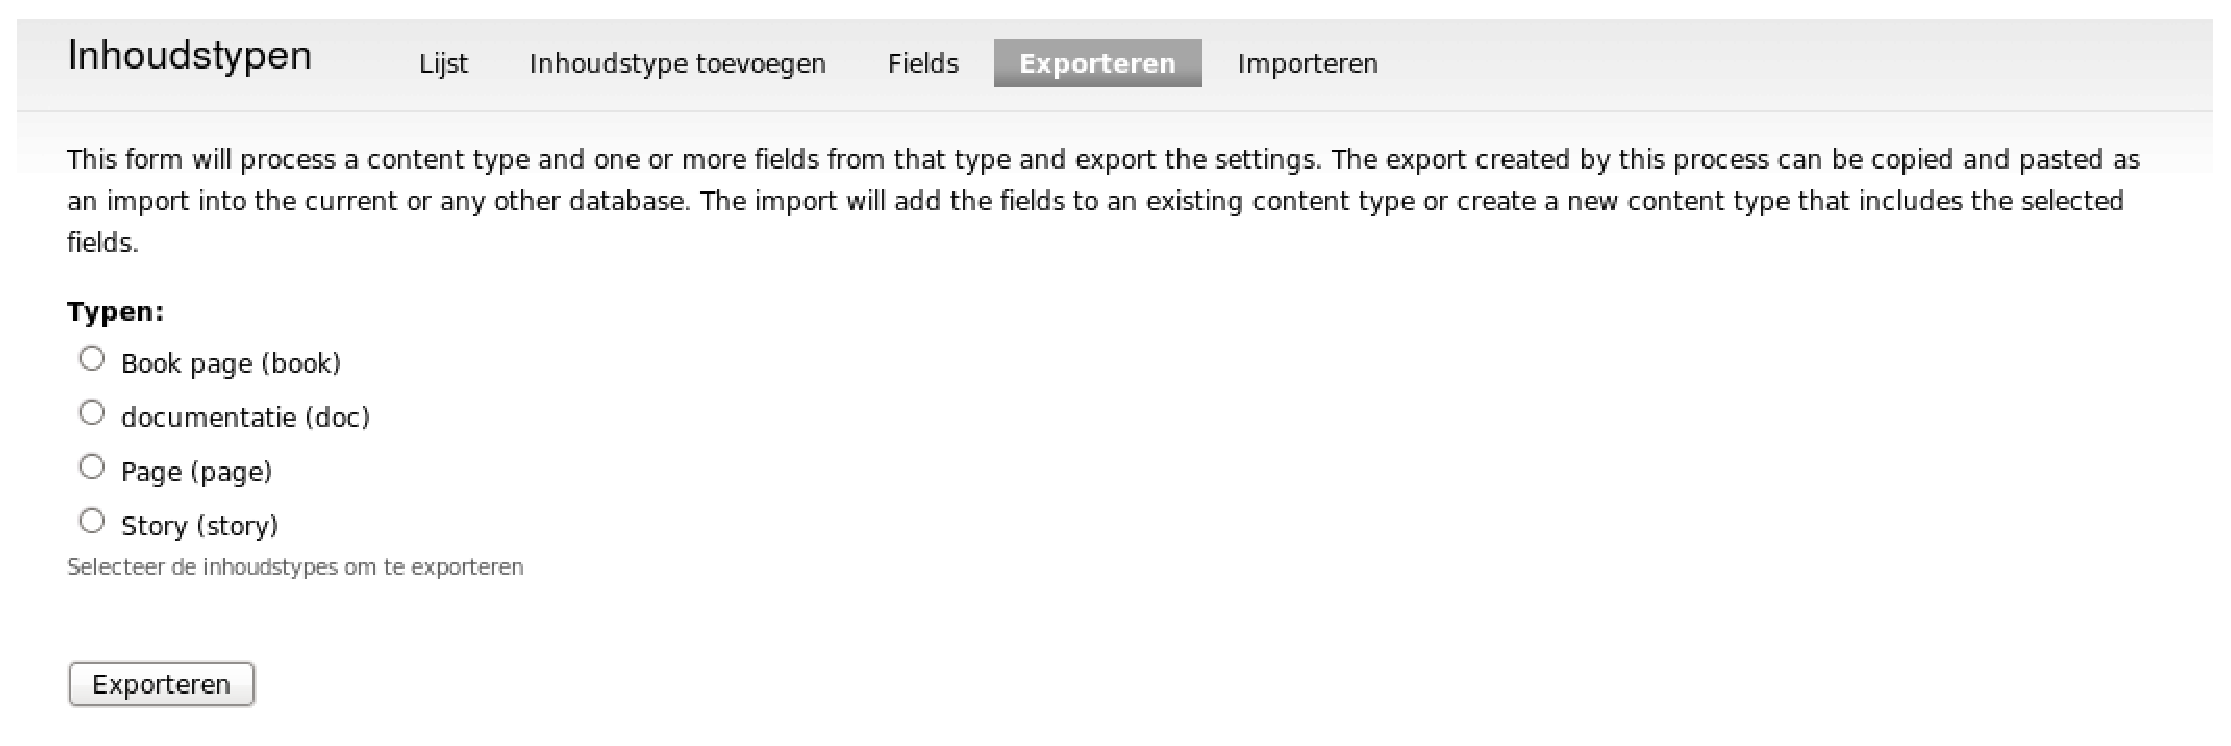
\includegraphics[scale=0.3,angle=0]{inhoudstypen-exporteren}
   \caption{inhoudstypen-exporteren.\label{white}}
 \end{figure}

\subsection{Importeren} \index{importeren}
Dit formulier zal veldinformatie importeren die zijn geexporteerd uit een ander inhoudstype of database.
Merk op dat velden niet kunnen worden gedupliceerd in hetzelfde inhoudstype, dus
ge\"importeerde velden zullen alleen worden toegevoegd als ze nog niet bestaan
in het geselecteerde inhoudstype. \begin{figure}[!h]
    \centering
   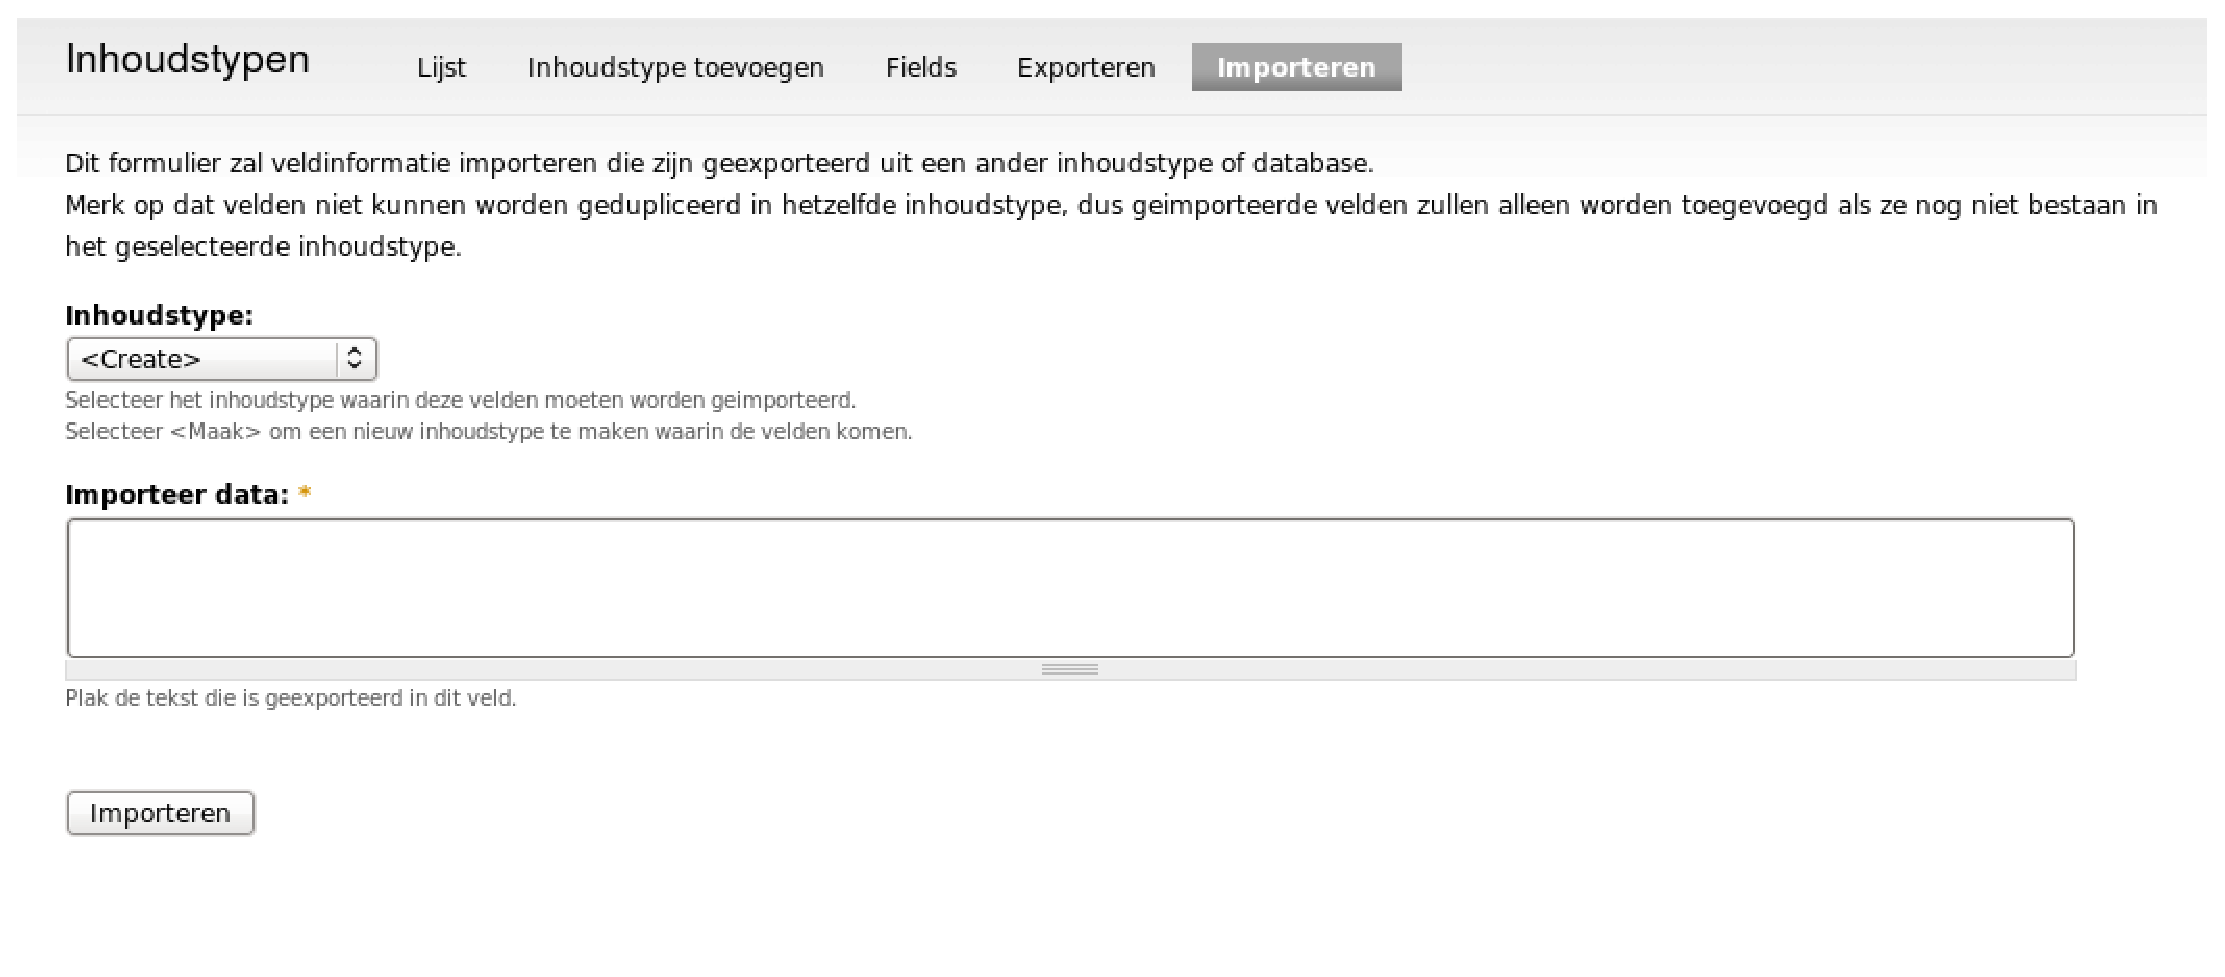
\includegraphics[scale=0.3,angle=0]{inhoudstypen-importeren}
   \caption{inhoudstypen-importeren.\label{white}}
 \end{figure}

\section{Instellingen voor inzendingen} \index{inzendingen}
Instellingen van inzendingen beheren zoals de lengte van het voorproefje,
verplichtte voorbeeldweergave \index{voorbeeldweergave} voor inzenden en het
aantal inzendingen op de voorpagina. \begin{figure}[!h]
    \centering
   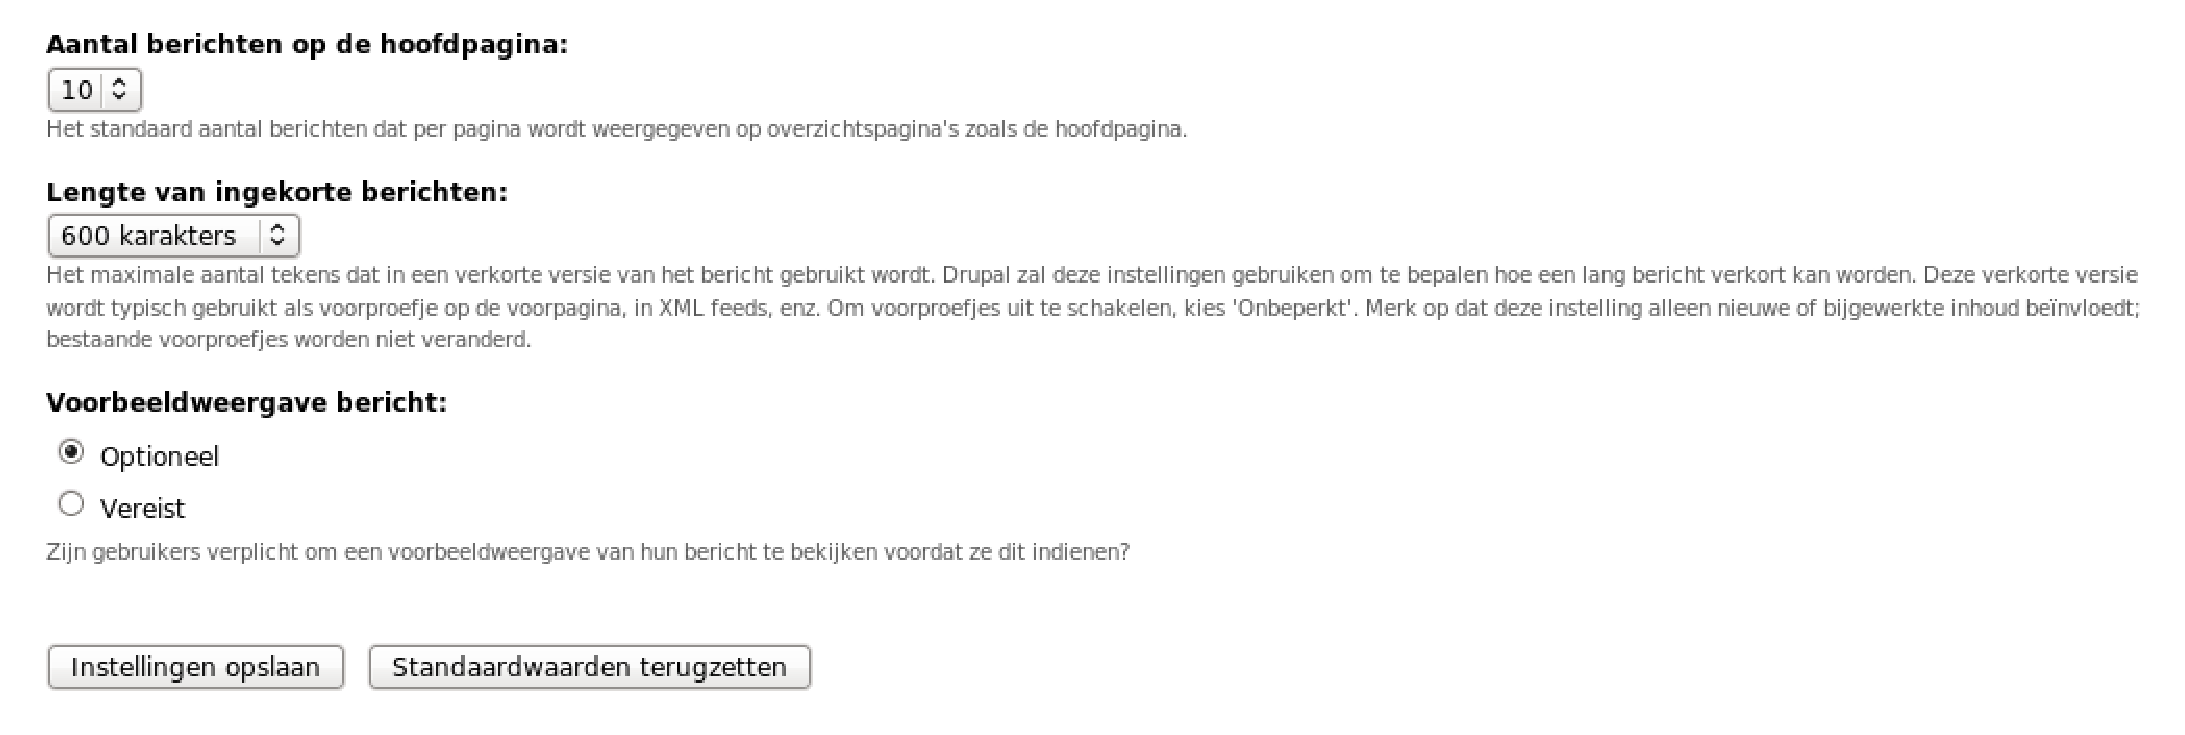
\includegraphics[scale=0.3,angle=0]{instellingen-inzendingen}
   \caption{instellingen-inzendingen.\label{white}}
 \end{figure}
\subsection{Node toegangsstatus} \index{toegangsstatus}
Wanneer er op de site problemen optreden met toegang tot de inhoud moet u de toegangsrechten-cache
opnieuw samenstellen. Mogelijke oorzaken voor toegangsproblemen zijn het uitschakelen van modules of
veranderingen in de toegangsrechten. Bij het opnieuw samenstellen van de cache worden alle rechten
verwijderd om te worden vervangen door rechten gebaseerd op actuele modules en instellingen.
\\
Het opnieuw samenstellen kan enige tijd in beslag nemen als de site veel inhoud bevat of als de
toegangsrechten complex zijn. Na afloop zullen alle berichten van de nieuwe toegangsrechten zijn voorzien.
\subsection{Aantal berichten op de hoofdpagina}
Het standaard aantal berichten dat per pagina wordt weergegeven op
overzichtspagina's zoals de hoofdpagina.
\subsection{Lengte van ingekorte berichten}
Het maximale aantal tekens dat in een verkorte versie van het bericht gebruikt
wordt. Drupal zal deze instellingen gebruiken om te bepalen hoe een lang bericht
verkort kan worden. Deze verkorte versie wordt typisch gebruikt als voorproefje op
de voorpagina, in XML feeds, enz. Om voorproefjes uit te schakelen, kies 'Onbeperkt'.
Merk op dat deze instelling alleen nieuwe of bijgewerkte inhoud be\"invloedt;
bestaande voorproefjes worden niet veranderd.
\subsection{Voorbeeldweergave bericht}
\begin{itemize}
\item Optioneel
\item Vereist
\end{itemize}
Zijn gebruikers verplicht om een voorbeeldweergave van hun bericht te bekijken
voordat ze dit indienen?

\section{RSS-publicatie} \index{rss-publicatie}
\begin{figure}[!h]
    \centering
   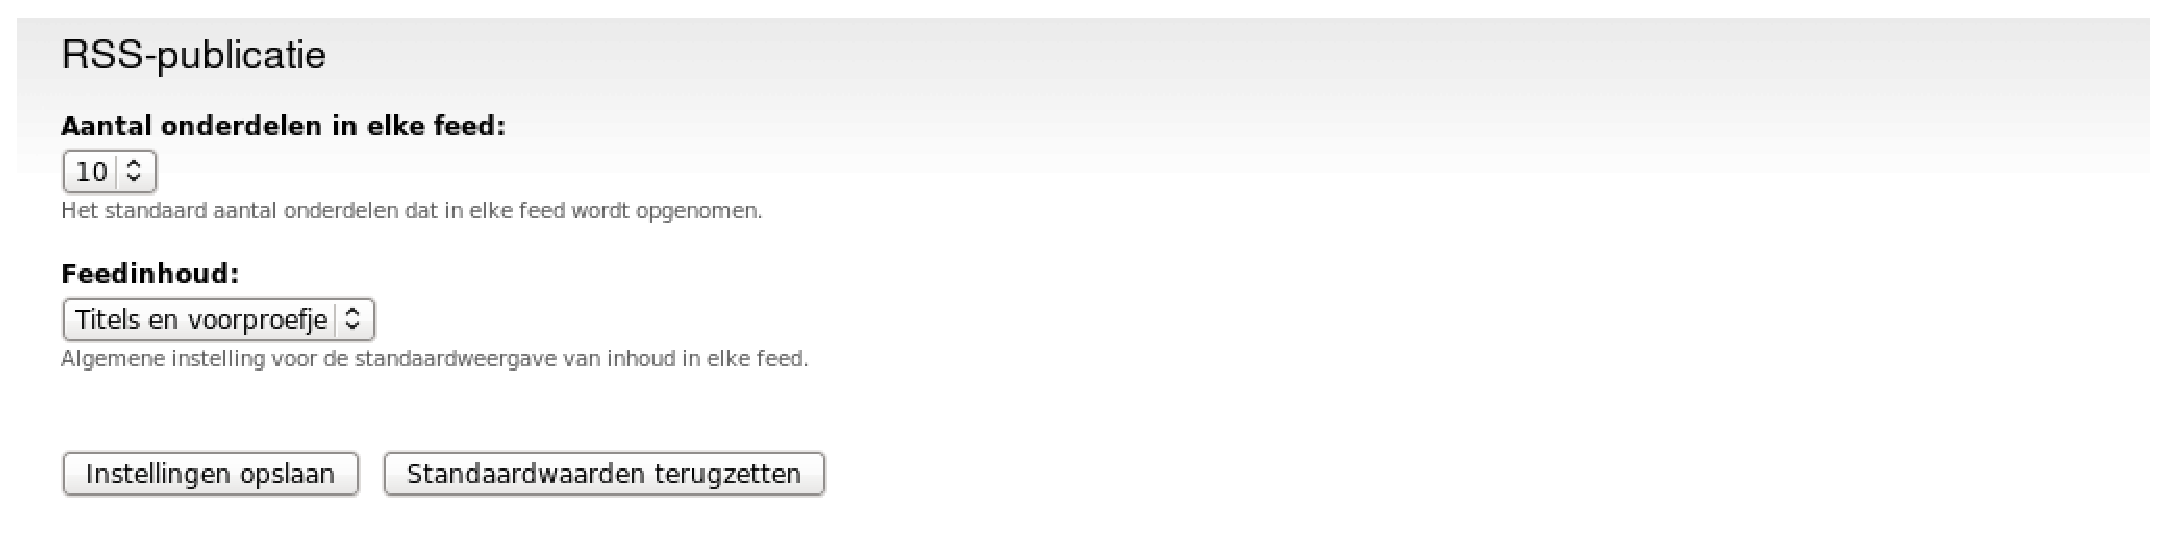
\includegraphics[scale=0.3,angle=0]{rss-publicatie}
   \caption{rss-publicatie.\label{white}}
 \end{figure}
Bepaal het aantal onderwerpen per feed en of feeds met titel, voorproefje of
volledige tekst worden weergegeven.

\section{Reacties} \index{reacties}
Reacties en de moderatiewachtrij voor reacties weergeven en wijzigen.
\subsection{Comment-module} \index{comment-module}
Met de Comment-module kunnen bezoekers reageren op uw bijdrage in een ad-hoc discussieforum.
Ieder inhoudstype kan Standaard reactie-instellingen hebben voor Lezen/Schrijven van een reactie
of de mogelijkheid tot reageren is Uitgeschakeld. Instellingen voor weergave van reacties en andere
reactie-instellingen kunnen ook per nodetype worden bepaald. Sommige weergave-instellingen zijn per gebruiker te bepalen.
\\
Reactierechten \index{reactierechten} worden toegekend per gebruikersrol en
worden gebruikt om te bepalen of anonieme bezoekers of gebruikers met andere rollen het recht hebben op een inzending te reageren. Als anonieme bezoekers het
recht hebben om te reageren, kan contactinformatie in een cookie op de computer van de bezoeker worden
opgeslagen voor gebruik bij volgende reacties. Als er geen vervolg-reacties zijn op een reactie kan de
auteur (optioneel) de eigen reactie wijzigen. De Comment-module gebruikt de zelfde invoerformaten en
HTML-tags als bij het aanmaken van andere inhoud beschikbaar zijn.
\subsection{Gepubliceerde reacties} \index{gepubliceerde reacties}
Een lijst van recente reacties op de site. Klik op het onderwerp om de reactie
te lezen, op de naam van de schrijver om de gebruikersinformatie van de schrijver
te bewerken, op 'bewerken' om de tekst te bewerken of op 'verwijderen' om de reactie te verwijderen.
\begin{figure}[!h]
    \centering
   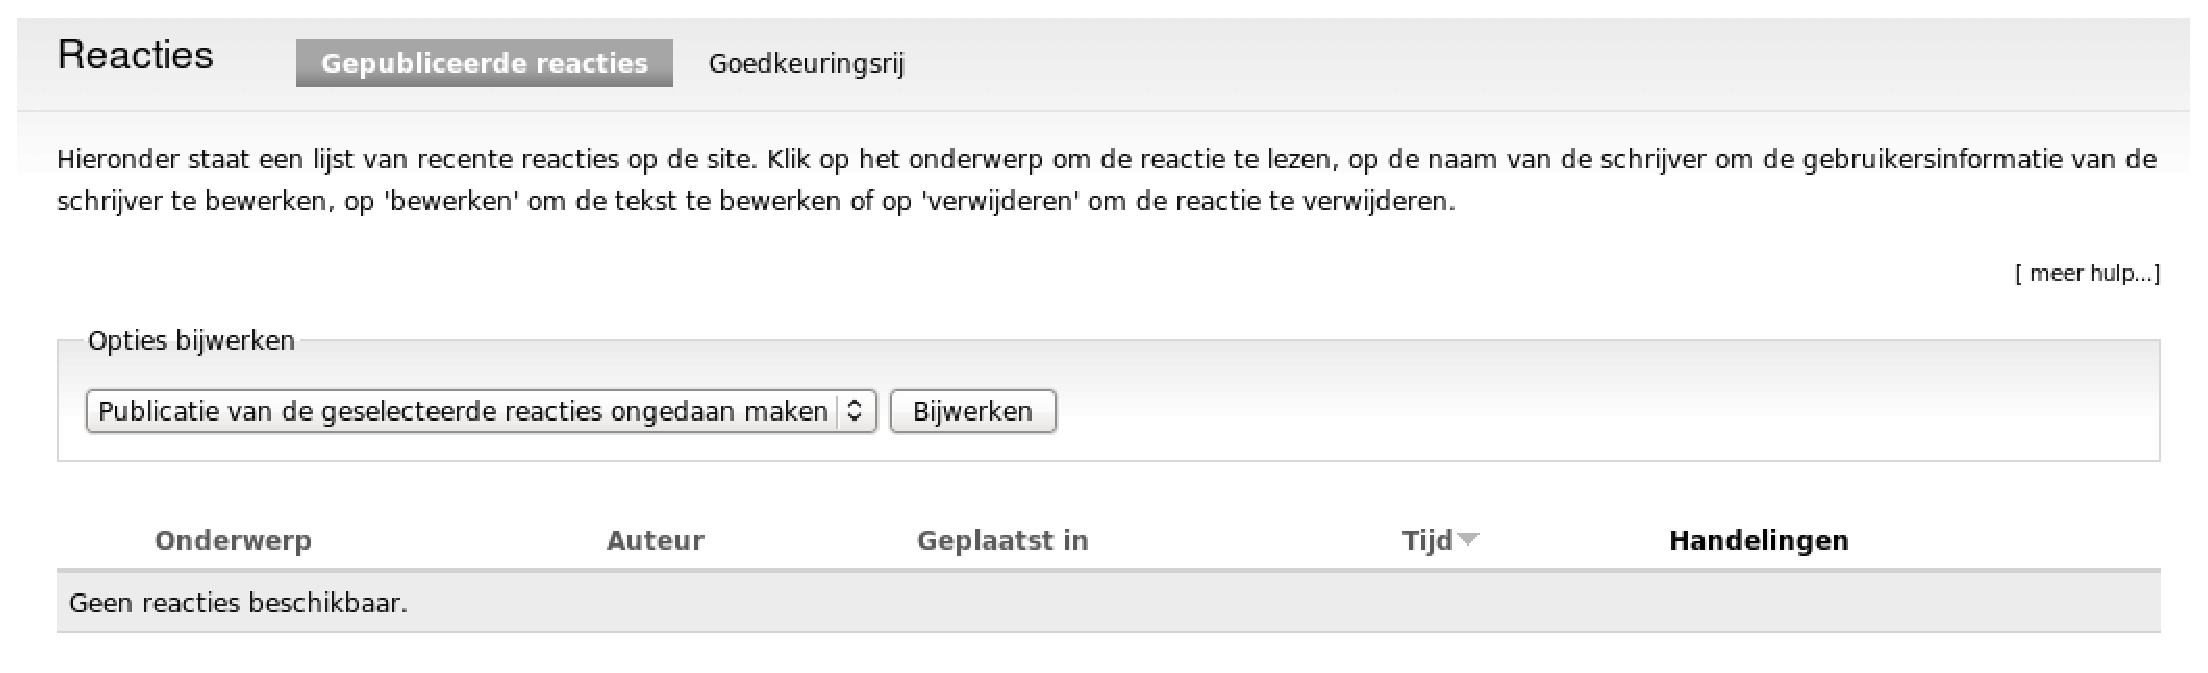
\includegraphics[scale=0.3,angle=0]{reacties-geplubliceerd}
   \caption{reacties-geplubliceerd.\label{white}}
 \end{figure}
\subsection{Goedkeuringsrij} \index{goedkeuringsrij}
Een lijst van recente reacties die moeten worden goedgekeurd. Klik op
'bewerken' en wijzig de 'moderatiestatus' \index{moderatiestatus} in Goedgekeurd
om een reactie goed te keuren. Klik op een onderwerp om de reactie te zien, op de naam van de schrijver om de gebruikersinformatie
te bewerken, op 'bewerken' om de tekst te bewerken en op 'verwijderen' om de
reactie te verwijderen. \begin{figure}[!h]
    \centering
   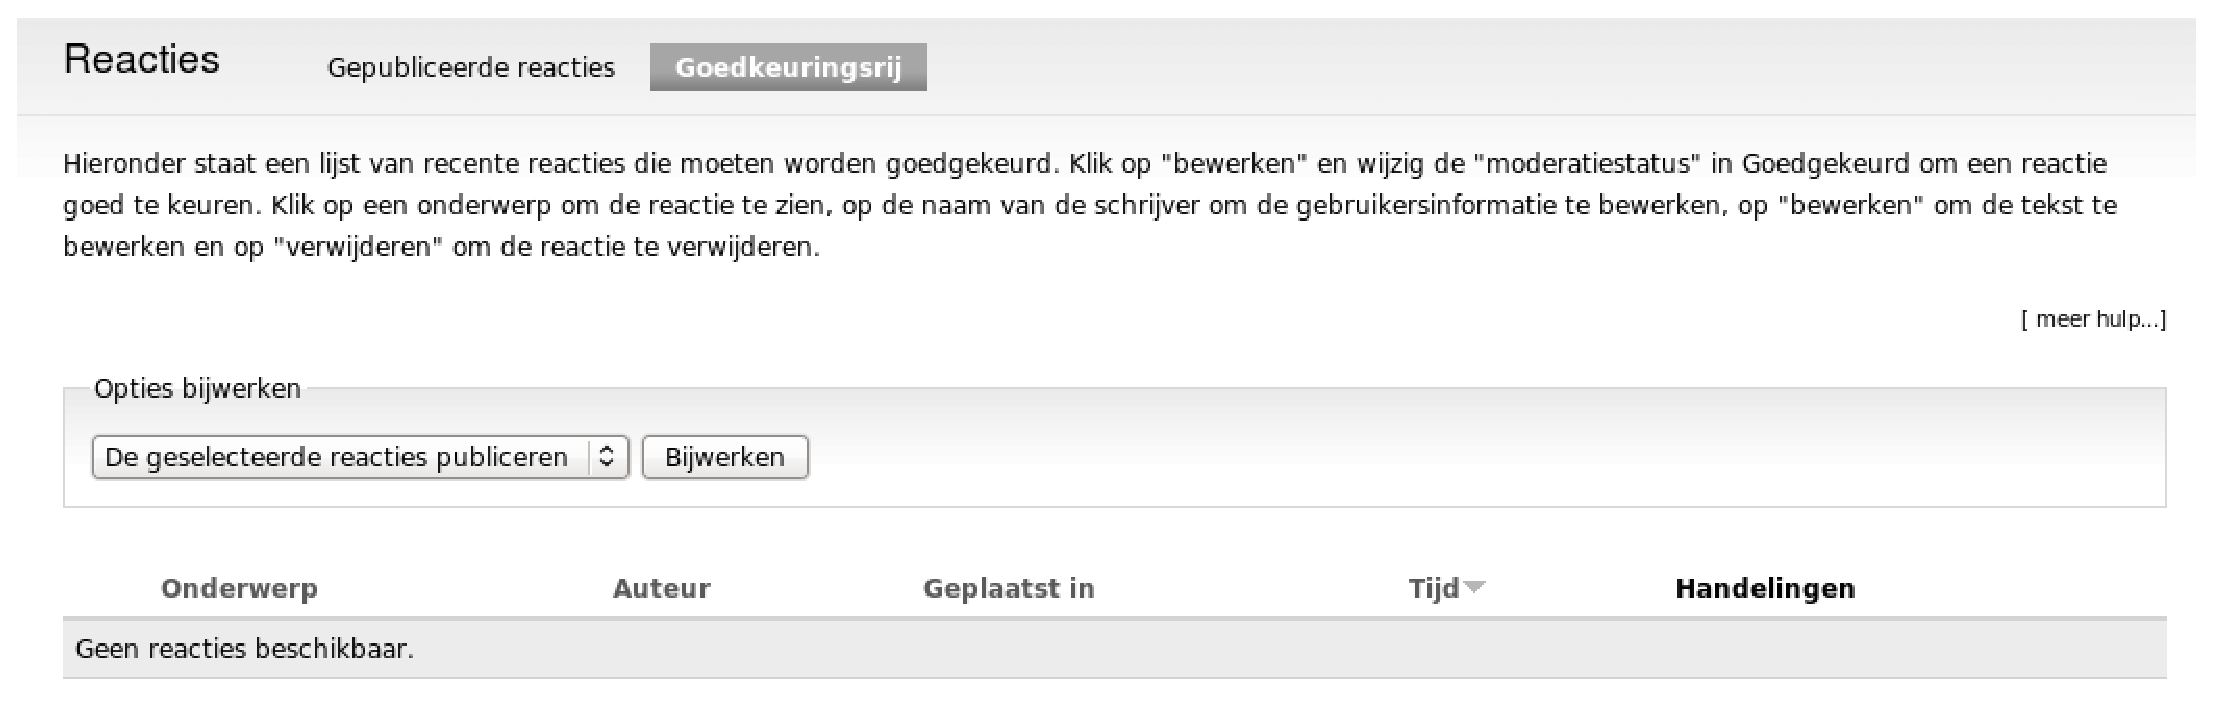
\includegraphics[scale=0.3,angle=0]{reacties-goedkeuringsrij}
   \caption{reacties-goedkeuringsrij.\label{white}}
 \end{figure}

\section{Taxonomie} \index{taxonomie}
Beheren van labelen \index{labelen}, categoriseren \index{categoriseren} en
classificeren \index{classificeren} van de website-inhoud.
\subparagraph{Taxonomy-module} \index{taxonomie-module}
Met de Taxonomy-module kunt u de inhoud van de website met behulp van verschillende
classificatie systemen categoriseren. Met 'Vrij labelen' kunnen gebruikers tijdens het
indienen van inhoud deze van zelf gekozen labels voorzien (deze methode wordt vaak in
blogs en community-sites toegepast). Met gecontroleerde woordenlijsten kunnen eenvoudige
lijsten, maar ook complexe hi\"erarchie\"en met meervoudige relaties tussen de termen, worden
samengesteld om inhoud te categoriseren. Deze methoden kunnen op verschilende inhoudstypen
worden toegepast en gecombineerd worden tot een krachtige en flexibele methode voor het
classificeren en presenteren van de website-inhoud.
\\
Wanneer u bijvoorbeeld een receptensite maakt, wilt u wellicht berichten classificeren op het
soort maaltijd en op bereidingstijd. Met een woordenlijst voor maaltijd \'en
voor bereidingstijd kunt u beide criteria onafhankelijk van elkaar gebruiken in plaats van voor elke mogelijke combinatie een nieuwe label aan te maken.
\begin{itemize}
\item Soort gerecht: Voorgerecht, Hoofdgerecht, Salade, Dessert
\item Bereidingstijd: 0-30 min., 30-60 min., 1-2 uur, meer dan 2 uur
\end{itemize}
Iedere taxonomie-term (in andere systemen ook wel 'categorie' of 'tag' genoemd) voorziet standaard
in een lijst van inzendingen met deze term en een bijbehorende RSS-feed. De URL's van deze lijsten
kunnen worden samengesteld om EN- en OF-lijsten te maken van inzendingen die van verschillende termen
zijn voorzien. In het voorbeeld van de receptensite kunnen eenvoudig pagina's gemaakt worden met alle
'Hoofdgerechten', '30 minuten' recepten of een samengestelde lijst '30 minuten hoofdgerechten en voorgerechten'
door gebruik te maken van losse of gecombineerde termen. Er is een groot aantal uitbreidingsmodules beschikbaar
waarmee u de functionaliteit van de kernmodules op het gebied van weergave en organisatie van termen kunt veranderen en uitbreiden.
\\
Op de beheerpagina kunnen termen hi\"erarchisch gerangschikt worden. Bijvoorbeeld landen rangschikken van onder regio's in de wereld.
Met de Taxonomy-module kunnen gegevens op geavanceerde wijze worden gerangschikt. Zoals bijvoorbeeld Turkije plaatsen onder
'Midden Oosten' \'en onder 'Europa'.
\\
De Taxonomy-module maakt het gebruik van synoniemen en gerelateerde termen mogelijk maar kent geen actieve ondersteuning hiervan.
Uitbreidingsmodules kunnen deze functies echter volledig benutten.
\subsection{Lijst}
Met de Taxonomy-module kunt u inhoud van de site classificeren met labels en
gecontroleerde termen. Het is een flexibel classificatie gereedschap met geavanceerde mogelijkheden.
Om te beginnen wordt een 'Woordenlijst' aangemaakt voor een groep van labels of termen.
U kunt één woordenlijst voor vrij-labelen voor alle termen aanmaken of verschillende gecontroleerde
woordenlijsten die ieder verschillende eigenschappen van de inhoud weergeven; Bijvoorbeeld: 'Landen' en 'Kleuren'.
\\
De onderstaande lijst kan gebruikt worden om de gebruikte woordenlijsten te controleren
en te configureren of om de termen (labels) daarin te beheren. Een woordenlijst is (optioneel)
gekoppeld aan een inhoudstype weergegeven in de kolom Type en wordt bij het aanmaken of bewerken
van een pagina van dit inhoudstype weergegeven. Wanneer meerdere woordenlijsten aan een zelfde
inhoudstype zijn gekoppeld worden deze in de onderstaande volgorde weergegeven. Om de volgorde
van de woordenlijsten aan te passen klik-sleept u een woordenlijst aan het handvat in de kolom
Naam naar een nieuwe positie in de lijst. (U klik-sleept het blok door met de muis boven het
handvatpictogram te klikken, vast te houden en de muis te verplaatsen.) Wijzigingen worden
pas opgeslagen wanneer u de knop Opslaan onderaan de pagina aanklikt.
\subsection{Woordenlijst toevoegen} \index{woordenlijst toevoegen}
\begin{figure}[!h]
    \centering
   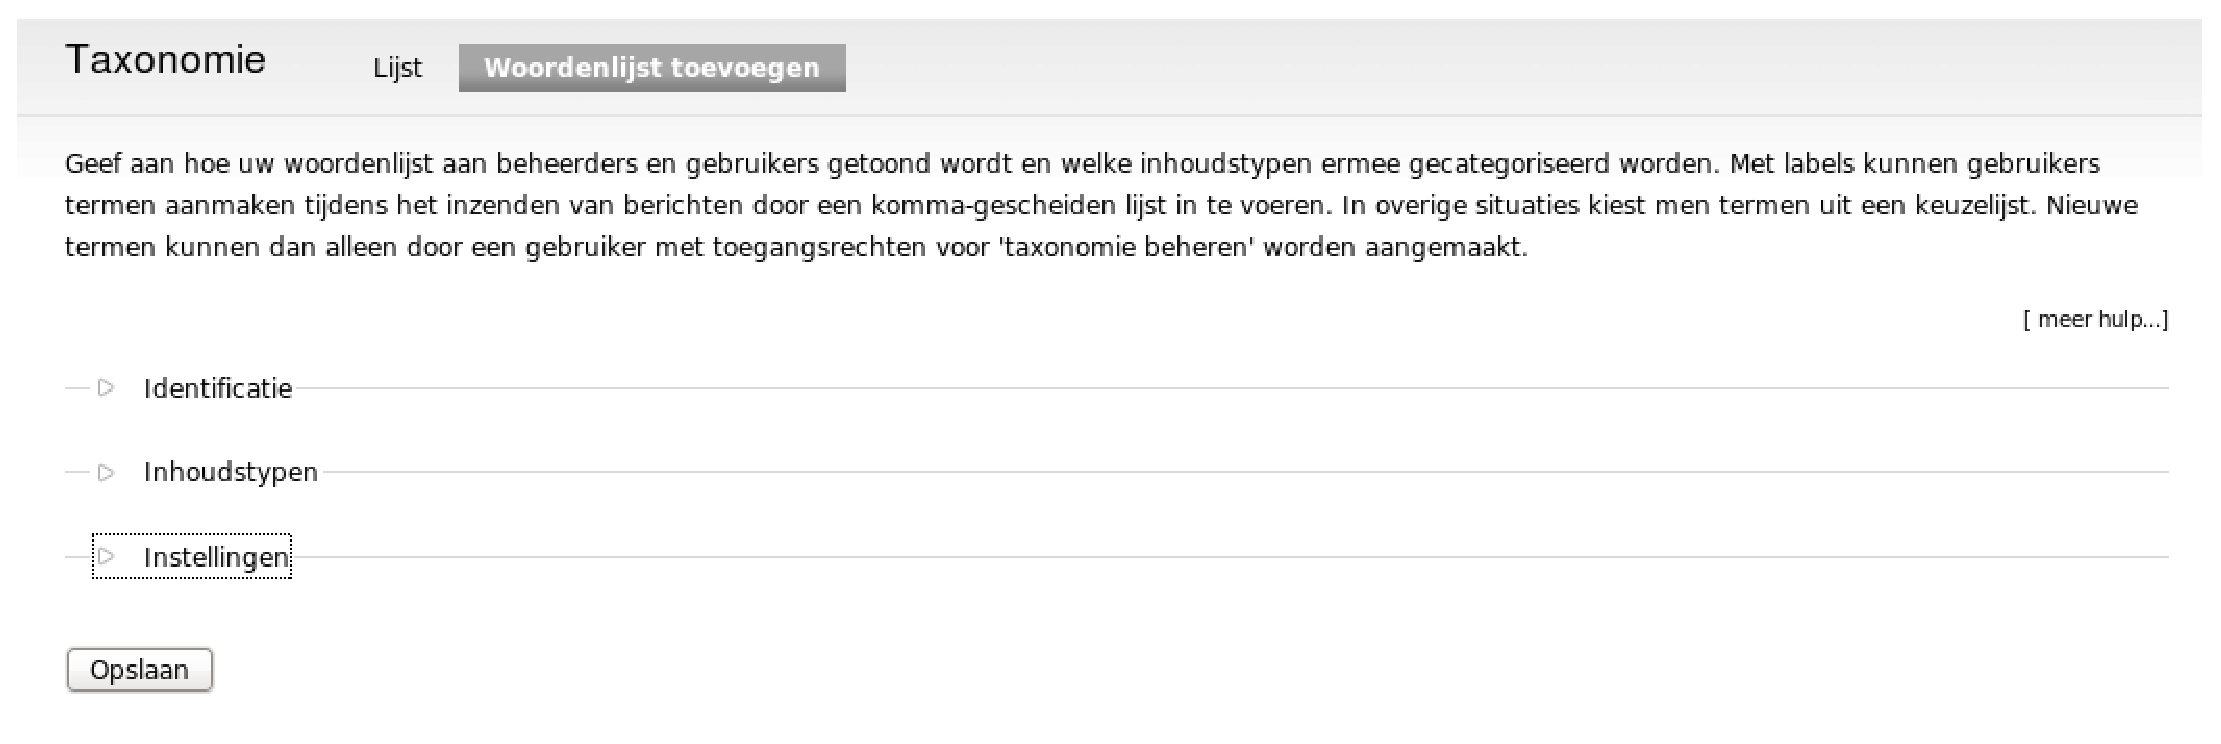
\includegraphics[scale=0.3,angle=0]{woordenlijst-toevoegen}
   \caption{woordenlijst-toevoegen.\label{white}}
 \end{figure}
Geef aan hoe uw woordenlijst aan beheerders en gebruikers getoond wordt en welke
inhoudstypen ermee gecategoriseerd worden. Met labels kunnen gebruikers termen aanmaken
tijdens het inzenden van berichten door een komma-gescheiden lijst in te voeren.
In overige situaties kiest men termen uit een keuzelijst. Nieuwe termen kunnen dan
alleen door een gebruiker met toegangsrechten voor 'taxonomie beheren' worden aangemaakt.
\subsubsection{Woordenlijst-identificatie} \index{identificatie woordenlijst}
\begin{itemize}
\item Naam van woordenlijst: De naam van deze woordenlijst. Bijvoorbeeld:''tags''
\item Beschrijving: Beschrijving van de woordenlijst; kan gebruikt worden door
modules.
\item Helptekst: Instructies voor de gebruiker bij het selecteren van termen.
Bijvoorbeeld: ''Voer een lijst in, gescheiden door komma's''.
\end{itemize}
\begin{figure}[!h]
    \centering
   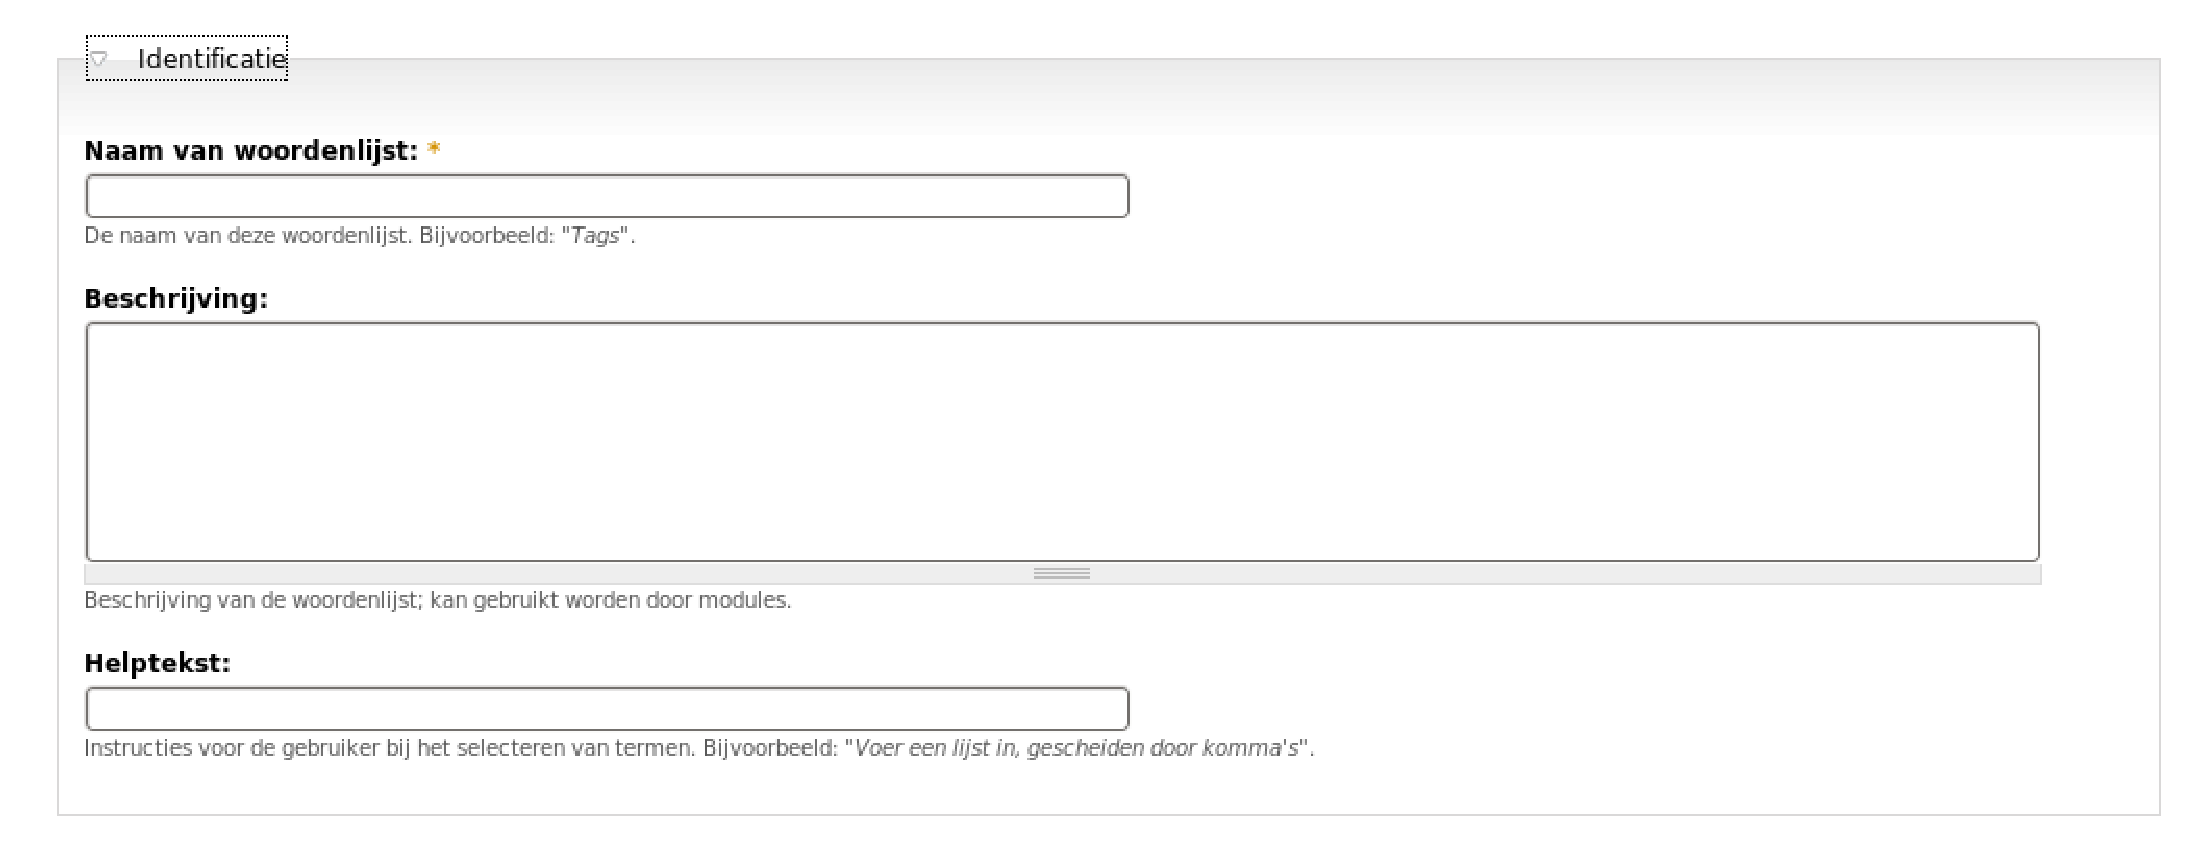
\includegraphics[scale=0.3,angle=0]{woordenlijst-identificatie}
   \caption{Woordenlijst-identificatie.\label{white}}
 \end{figure}
 \subsubsection{Woordenlijst-inhoudstypen}
 Gebruik de woordenlijst om inhoudstypen te categoriseren.
\begin{itemize}
\item Book page
\item Page
\item Story
\item \ldots
\end{itemize}
\begin{figure}[!h]
    \centering
   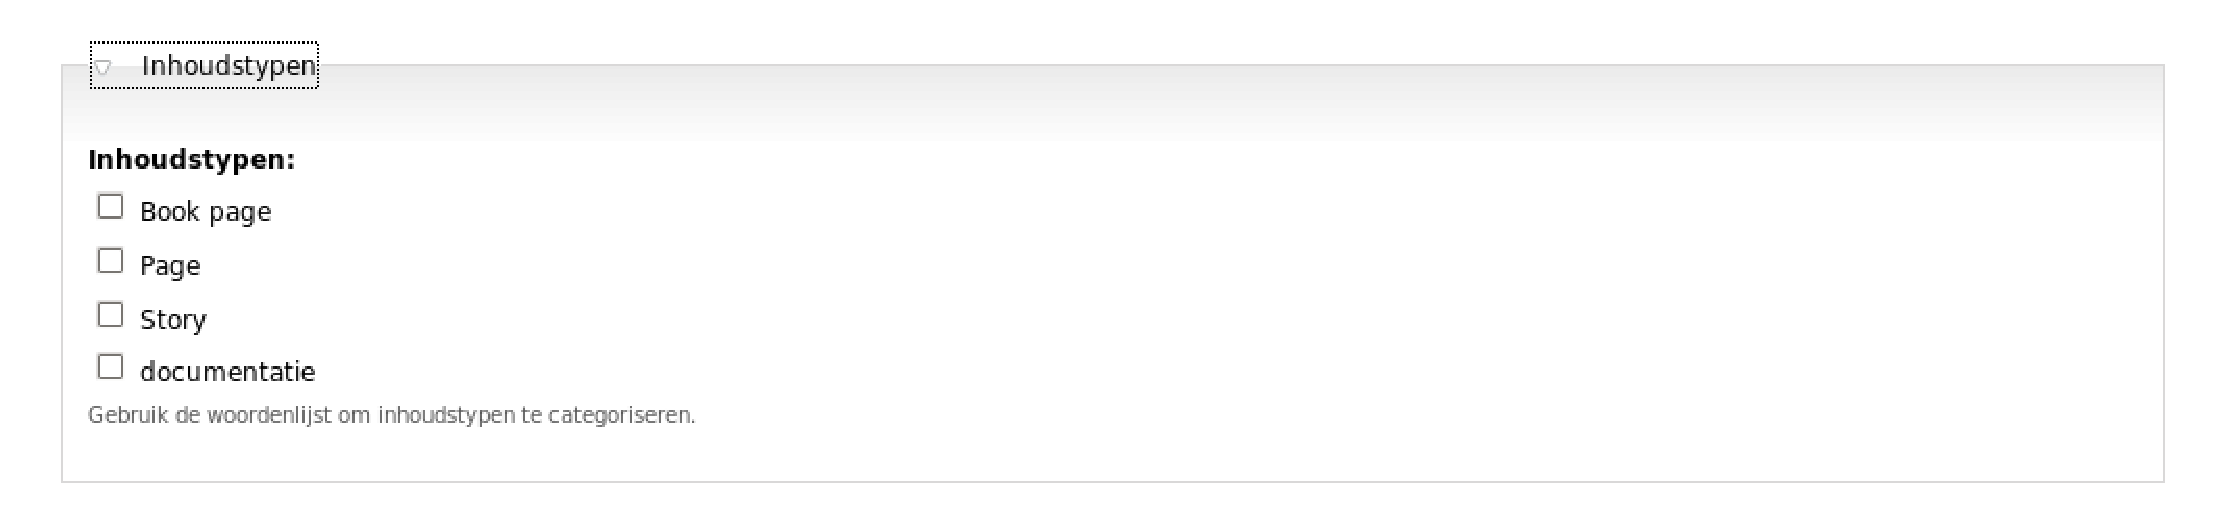
\includegraphics[scale=0.3,angle=0]{woordenlijst-inhoudstypen}
   \caption{woordenlijst-inhoudstypen.\label{white}}
 \end{figure}

 \subsubsection{Woordenlijst-instellingen} \index{instellingen woordenlijst}
 \begin{itemize}
\item Labels: Termen worden aangemaakt wanneer gebruikers een door komma's
gescheiden lijst indienen.
\item Meervoudige selectie: Inzendingen mogen meer dan \'e\'en term uit deze
woordenlijst bevatten (altijd geldig voor labels).
\item Vereist: Inzendingen moeten minimaal \'e\'en term uit deze woordenlijst
bevatten.
\end{itemize}
\begin{figure}[!h]
    \centering
   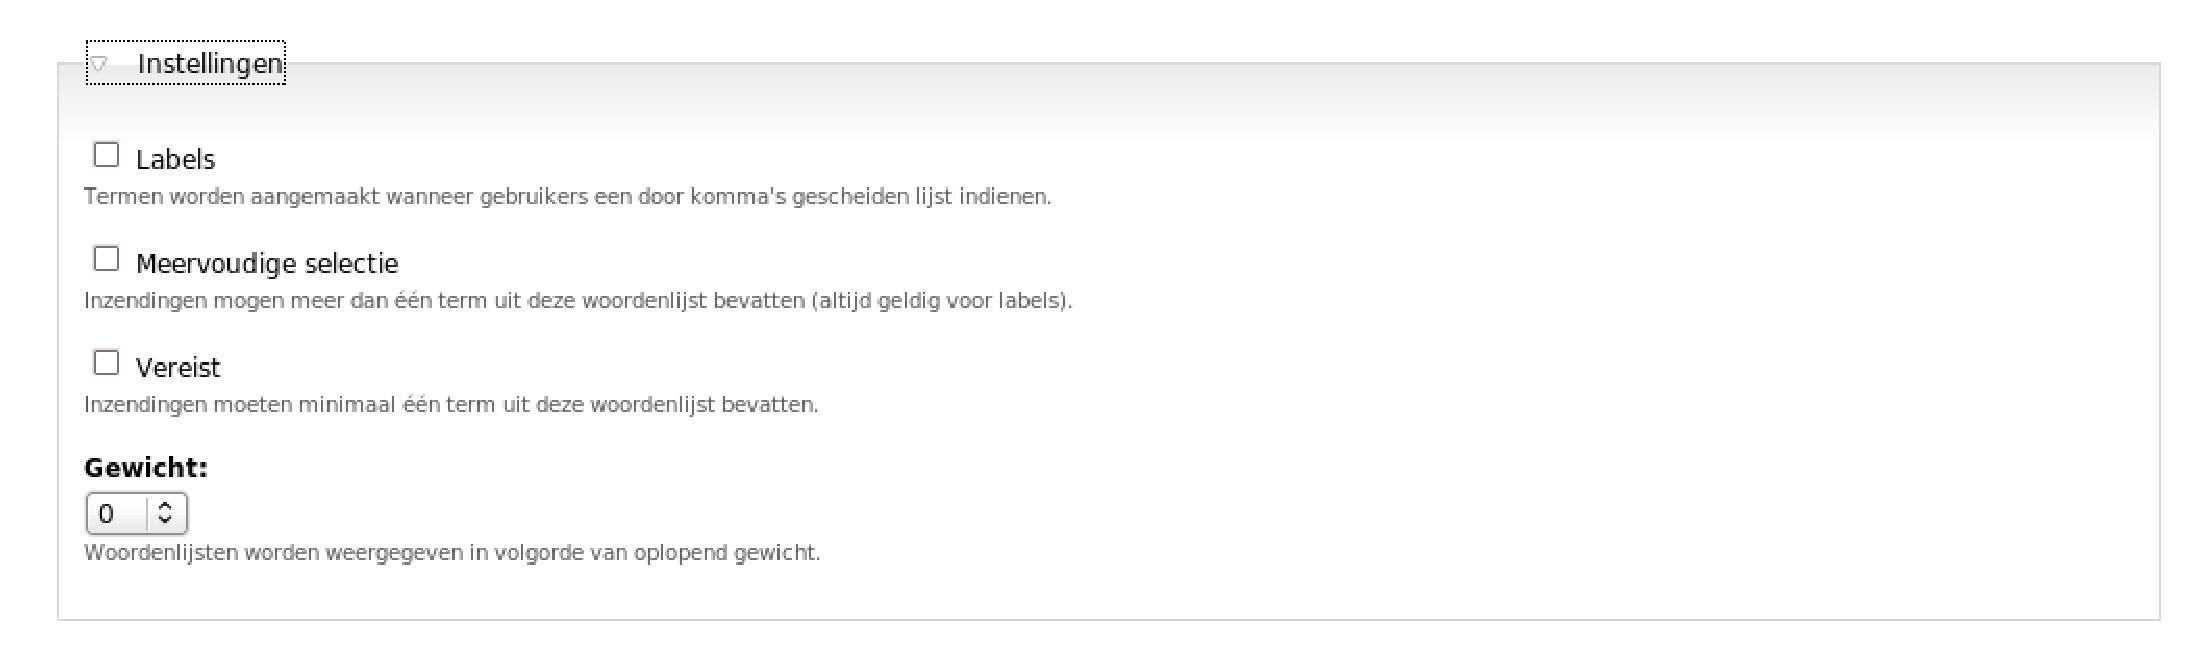
\includegraphics[scale=0.3,angle=0]{woordenlijst-instellingen}
   \caption{Woordenlijst-instellingen.\label{white}}
 \end{figure}